
\documentclass[conference]{IEEEtran}
\usepackage{cite}
\usepackage{amsmath,amssymb,amsfonts}
\usepackage{algorithmic}
\usepackage{graphicx}
\usepackage{textcomp}
\usepackage{xcolor}
\usepackage{hyperref}
\hypersetup{
    colorlinks=true,
    urlcolor=blue,
    citecolor=black
}
\urlstyle{same}
\def\BibTeX{{\rm B\kern-.05em{\sc i\kern-.025em b}\kern-.08em
    T\kern-.1667em\lower.7ex\hbox{E}\kern-.125emX}}
\usepackage{xparse}
\usepackage{graphicx}
\graphicspath{ {./images} }
\NewDocumentCommand{\code}{v}{%
\texttt{\textcolor{black}{#1}}%
}

\begin{document}

\title{ Quantum with Qiskit \\
{\footnotesize A guide to the python package}
}

\author{\IEEEauthorblockN{Parish Wolfe}
\IEEEauthorblockA{\textit{Dept. of Computer Science} \\
\textit{Vanderbilt University)}\\
Raleigh, NC \\
parish.m.wolfe@vanderbilt.edu
}}

\maketitle

\begin{abstract}
IBM Qiskit is contains interfaces to quantum infrastructure with built in algorithms for domain specific uses.
\end{abstract}

\begin{IEEEkeywords}
quantum computing, quantum programming, qubit, gate, python, pip, 
\end{IEEEkeywords}

\section{Introduction}
International Business Machines or IBM has created great products over the years, from the mainframe computer to IBM Watson, while simultaneously delivering hardware from their parent company, Lenovo. 
In March of 2017, IBM started an open source python project known as Qiskit.
This project is under the Apache License 2.0, which allows for use with few stipulations \cite{b1}.
The first commit was on Friday, March 3rd 2017 at 6:09 PM Eastern Standard Time by Physics Researcher Jay Gambetta, who continues to work as an IBM Fellow and Vice President of IBM Quantum.
Since its inception, the project has grown massively in significance at both IBM and in the field of quantum computing. 
Qiskit currently sits at the top of quantum computing frameworks in terms of popularity. 
Due to the combined expertise of hardware and software at IBM, the company has long held the title of the most popular quantum computing framework.
IBM has been making strides in quantum hardware.
Recently, they announced the "Eagle" quantum processor, which holds 127 qubits \cite{b2}.
The metrics that IBM looks at to measure their hardware success include: quantity of qubits, quality by quantum volume, and speed in circuit layer operations per second.
With all this success in quantum hardware, there is a need for software to utilize all the advances.
This is where Qiskit fills the void. 

\section{Qiskit}
Qiskit is a quantum circut python package that has several add-ons available. These will be discussed in detail later on. 
Qiskit also includes a transpiler that converts qiskit code into a quantum circuit capable of running on any quantum backend and on real hardware. 
IBM offers the "IBM Quantum Lab" which is a Jupyter Notebook environment, that allows one to connect to a quantum service that runs the code on a real quantum computer.
A quantum simulator, Aer, is provided as well, which makes it easy to get started \cite{b4}.
Aer will be discussed in more detail in a later section. 
IBM offers the IMB Quantum Lab, which is a jupyter notebook environment that is seamlessly integrated with IBM's quantum backends via http API.
Various quantum hardware providers are available through qiskit's backend service \cite{b5}. 
The basic elements of quantum programming are provided in the terra repository. 
This library is installed when one runs \code{pip install qiskit} along with Aer. 
Quantum programming with Terra is discussed in more detail in a later section. 
Terra includes jupyter tools and visualizations that help out when working with jupyter notebook. 
Qiskit supports all major platforms including Linux, macOS, and Windows. 

\section{Terra}
Terra contains the core functionality of qiskit quantum programming. 
All other add-on packages use Terra as a dependency. 
This package contains \code{qiskit.circuit} which contains all the building blocks for creating a quantum circuit. 

\subsection{Registers}
\code{qiskit.circuit.ClassicalRegister} can be instantiated with either a size or number of bits to store data, prior to using it in the quantum circuit.
The classical register can be compared to a traditional byte, though the size can be larger than a byte.
The \code{quiskit.circuit.QuantumRegister} method is how qubits are instantiated.
Many qubits can be created at one time with the quantum register, with the size parameter, which has a default of one. 
Like the classical register, the quantum register can also be instantiated with a bit parameter as well as an optional name.
Instantiating these objects is not necessary though, because the \code{qiskit.circuit.QuantumCircuit} object can instantiate these for you when the object itself is instantiated. 
The first two parameters of \code{QuantumCircuit(2,3)} are the number of qubits to instantiate and the number of classical bits to instantiate.
In the example above, calling this constructor would instantiate \code{QuantumRegister(2)} and \code{ClassicalRegister(3)}. 

\subsection{Quantum Circuits}
Following the creation of the circuit object, quantum gates can be added to the circuit by calling class methods on the \code{QuantumCircuit} object. 
For example, a Hadamard Gate or H gate can be added to the circuit by calling \code{qc.h} where \code{qc} is the \code{QuantumCircuit} object. 
All the common Gates are available as a single letter method. 
Pauli X, Pauli Y, and Pauli Z gates are available as methods \code{qc.x}, \code{qc.y}, and \code{qc.z}.
A phase gate S can be applied with the \code{qc.s}, and performs a pi over 2 phase and is called a P gate in some languages.
CNOT can be applied with either \code{qc.cx} or \code{qc.cnot}. 
This helps qiskit maintain equilibrium with other quantum languages like Microsoft Q\#. 
A comprehensive list of ready-made available gates can be found in the qiskit documentation \cite{b6}.
Each gate method listed requires parameters of which qubit or qubits will apply the transformation to. 
The circuit object also includes methods for control flow logic like \code{if_else}, and \code{while_loop} \cite{b7}. Control flow logic can be seen in figure \ref{fig:conditional}.
\begin{figure}
    \centering
\begin{verbatim}
from qiskit.circuit import *
bits = [Qubit(), Qubit(), Clbit()]
qc = QuantumCircuit(bits)
qc.h(0)
qc.cx(0, 1)
qc.measure(0, 0)
with qc.if_test((bits[2], 0)) as else_:
    qc.h(0)
with else_:
    qc.x(0)
\end{verbatim}
    \caption{Conditional logic in a quantum circuit}
    \label{fig:conditional}
\end{figure}

\subsection{Utilities}
A useful method for creating these applications in a jupyter notebook is the \code{qc.draw()} method.
This will display a graph of the circuit as it stands at that point in the code. 
This allows for debugging and is analogous to using a \code{print()} statement to see the contents of variables. 
Outside of the circut object, there are many tools and utilities available in the Terra package. 
Some of these include \code{qiskit.tools.jupyter} which has a progress bar, a function to display detailed backend information, and a job watcher. 
\code{qiskit.tools} includes a \code{job_monitor}, \code{backend_monitor}, and a \code{backend_overview} method to check the status of an actively running quantum circuit. 
\code{qiskit.utils} has a plethora of functionality like a \code{local_hardware_info} function to determine if the machine has quantum architecture on-board. 
Other functions in the utils subpackage are algorithm utilities to check if various dependencies are installed as well as dependency checkers for external packages like Seaborn.

\subsection{Providers}
A provider in the context of qiskit is an interface to a real quantum computer. 
All of these would be over the cloud, unless one has an actual quantum computer. 
The \code{qiskit.providers} subpackage \textbf{\textit{provides}} a \code{Backend} object that is used by the quantum circuit to run.
The package has support for a custom provider as well, so that new quantum companies can interface with qiskit as well. 
The transpiler \code{qiskit.transpiler} is used behind the scenes by qiskit to convert the high level python code into machine readable quantum code. See figure \ref{fig:transpile} for more details on this process \code{b8}.

\begin{figure}
    \centering
    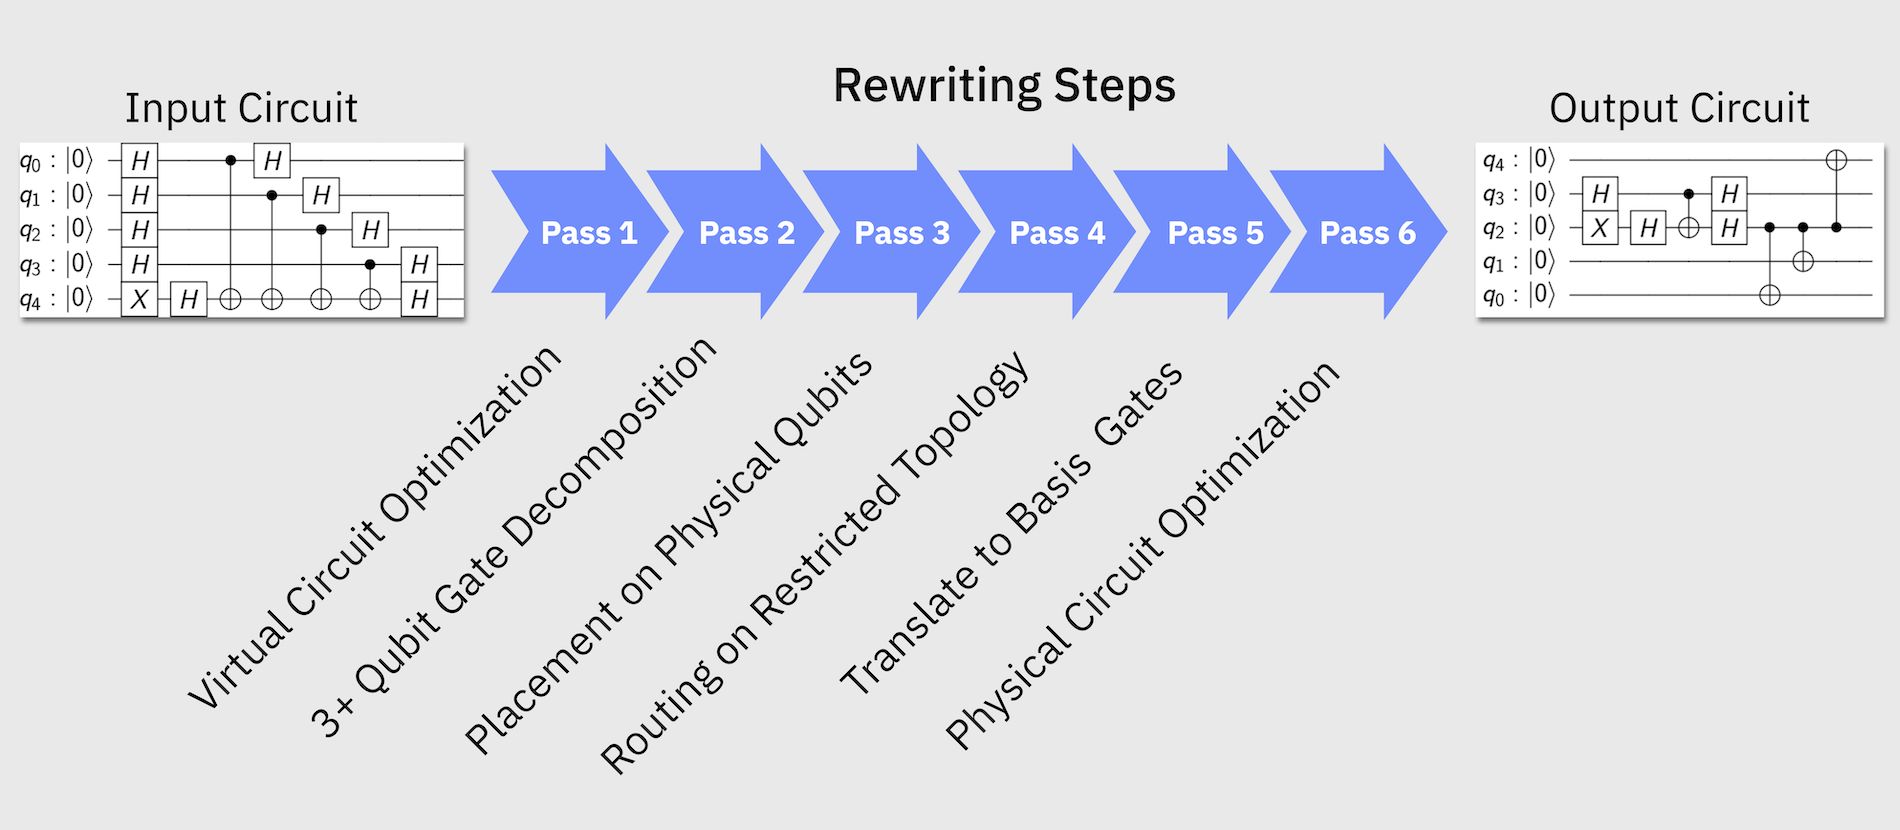
\includegraphics[width=\linewidth]{images/transpiling_core_steps.png}
    \caption{Transpiling core steps}
    \label{fig:transpile}
\end{figure}

\section{Aer}
Methods to connect to real quantum hardware reside in Qiskit Terra; simulated hardware methods are found in Aer.
Pronounced "air," this subpackage also allows for providers. 
The difference is that Aer providers are simulated quantum hardware and normal providers are for bona-fide real quantum hardware. 
The main entrypoint for Aer is \code{qiskit_aer.AerProvider.get_backend}. 
Depending on how you import this, you may be able to call this with \code{Aer.get_backend()}.
The default behavior of Aer is to supply the result of the quantum circuit with no noise. 
This behavior can be changed with a noise model \cite{b9}. 
A good number of quantum error functions are supplied out of the box, allowing for noise to be applied with a predictable error rate. 
Some of the built-in noise functions include \code{qiskit_aer.noise.pauli_error}, \code{qiskit_aer.noise.depolarizing_error}, \code{qiskit_aer.noise.mixed_unitary_error}, and many more. 
The ability to create a custom noise model is available too, if the supplied error models are unsatisfactory for one's use case. 
A more advanced use case of this module is \code{qiskit_aer.library}, which allows the user to modify the instruction set used by the transpiler. 
This object has very low level methods like \code{qiskit_aer.library.set_statevector} which allows the user to manipulate the vector state directly.
Modifiers for the density matrix and the clifford stabilizer state are in this subpackage as well. 
There are included utilities in Aer as well, like the ability to parallelize operations with an threadpool and api to dask \cite{b10}.
Dask is a library for parallel computing and is installed by default in anaconda. 
Quantum computers are much faster than classical computing infrastructure, so parallel approaches on the simulator can speed up complex circuits significantly.

\section{Domain Specific Uses}
Qiskit offers subpackages that are related to specific uses of quantum technology. 
These four use cases are Machine Learning, Nature, Finance, and Optimization. 
The benefit of of these domain specific packages are that they include built-in quantum algorithms for that use. 

\subsection{Machine Learning}
Subpackages like the qiskit machine learning are installed with pip add-on syntax.
\begin{verbatim}
pip install qiskit[machine-learning]
\end{verbatim}
There are two additional packages that are valuable in this space that can be installed in a similar fashion.
One of these packages is particularly useful, and that is a connector to PyTorch. 
The other is an integration with \code{scipy.sparse}.
\begin{verbatim}
pip install qiskit-machine-learning[torch]
pip install qiskit-machine-learning[sparse]
\end{verbatim}
Machine learning classification problems can be solved with the \code{NeuralNetworkClassifier} class. 
This class is compatible with Scikit-Learn and requires a \code{qml.neural_networks.NeuralNetwork} instance to be passed in as a parameter where \code{qiskit_machine_learning} is imported as \code{qml}. 
Similarly, the package has a \code{NeuralNetworkRegressor} class and has all the expected class methods such as \code{.fit(X,y)}, \code{.predict(X)}, and \code{.score(X, y[sample_weight])} \cite{b11}.
Distribution learning algorithms are available as well. 
The package is fully featured and can handle many different types of machine learning workflows. 

\subsection{Nature}
The nature package is primarily concerned with solving quantum mechanics natural science problems \cite{b13}. 
Not unlike the Machine learning package, Nature can be installed with pip.
\begin{verbatim}
pip install qiskit[nature]
\end{verbatim}
Some of the algorithms that come with the package are \code{ExcitedStatesSolver}, \code{EigensolverFactory}, \code{GroundStateSolver}, and \code{BOPESSampler} for potential energy.
Problems such as protein folding can be solved with the algorithms in this package. 
Additionally, thermodynamics observables can be found. 
This package deals in known difficult algorithms and formulas, and can solve these tough problems with ease. 

\subsection{Finance}
Aptly named, the finance package aims to perform calculations on stocks and securities so that profit can be maximised by predicting prices in the most accurate manner possible \cite{b14}.
\begin{verbatim}
pip install qiskit[finance]
\end{verbatim}
The above pip command will install the package in question. 
Portfolio optimization is one use case for the qiskit finance package. 
This involves an optimization problem with many inputs and provides the optimal balance between those assets to maximize returns. 
This boils down to a quadratic equation with many inputs, an area where quantum technology excels. 
The \code{qiskit_finance.data_providers} makes it easy to get real-time stock data on demand.
Several providers are already supported including NASDAQ DataOnDemand, Wikipedia, and Yahoo to name a few. 
Functionality to create one's own data provider exists as well. 
Fixed income problems, European options, and general estimation, and credit risk solvers are ready made in the package. 
As quantum technology progresses, this package is likely to see significant development in coming years. 

\subsection{Optimization}
The final subpackage available from qiskit is optimization \cite{b12}. 
This subpackage can be installed with pip similar to the others. 
\begin{verbatim}
pip install qiskit[optimization]
\end{verbatim}
The optimization package houses many of the textbook quantum algorithms, like grover optimization. 
This subpackage contains similar code to the finance package to solve quadratic problems. 
However, the pre-made algorithms are targeting mathematics and general uses, instead of finance. 
Some more advanced and specialty use cases are included here as well, such as an algorithm specific to vehicle routing. 
The optimization package is truly the miscellaneous area for qiskit, as there is an application for "Bin Packing" which calculates the most efficient way to "tetris" objects into a confined space. 
The \code{BinPacking} class can be readily imported from \code{qiskit_optimization.applications}.
Within \code{qiskit_optimization.algorithms} there are numerous optimizers with inputs for a wide array of problem types. 


\section{Conclusion}
Currently, IMB Qiskit leads the pack in the amount of information published on the topic of quantum technology. 
They have invested millions in quantum technology and intend to invest even more \cite{b15}. 
Plans for new investment include ongoing development in Qiskit's already comprehensive set up subpackages.
While the arms race for quantum technology heats up between competitors, some companies like IBM are playing nice with others. 
IBM and LG have set up an arrangement where LG can access IBM's quantum infrastructure \cite{b15}. 
Cooperation and collaboration among hardware manufacturers is sure to bring about breakthroughs at a faster pace.
With the pace of technology advancements, the quantum future is likely right around the corner. 

\begin{thebibliography}{00}
\bibitem{b5}How to Install Qiskit - Users. YouTube, 2022. Availble: \href{https://www.youtube.com/watch?v=1kRfHNUbkrg&list=PLOFEBzvs-VvpHs84vFdRVIl3Wlg81j8_x}{https://www.youtube.com/watch?v=1kRfHNUbkrg&list=PLOFEBzvs-VvpHs84vFdRVIl3Wlg81j8_x}
\bibitem{b15}N. Deslandes, “IBM expands quantum ecosystem with Quantinuum Investment,” TechInformed, 30-Aug-2022. [Online]. Available: \href{https://techinformed.com/ibm-expands-quantum-ecosystem-with-quantinuum-investment/}{https://techinformed.com/ibm-expands-quantum-ecosystem-with-quantinuum-investment/}. [Accessed: 05-Nov-2022]. 
\bibitem{b11}“Neuralnetworkregressor,” NeuralNetworkRegressor - Qiskit Machine Learning 0.4.0 documentation. [Online]. Available: \href{https://qiskit.org/documentation/machine-learning/stubs/qiskit_machine_learning.algorithms.NeuralNetworkRegressor.html?highlight=regression}{https://qiskit.org/documentation/machine-learning/stubs/qiskit_machine_learning.algorithms.NeuralNetworkRegressor.html?highlight=regression}. [Accessed: 05-Nov-2022]. 
\bibitem{b9}“Noise models (qiskit\_aer.noise),” Noise Models (qiskit\_aer.noise) - Qiskit 0.39.2 documentation. [Online]. Available: \href{https://qiskit.org/documentation/apidoc/aer_noise.html}{https://qiskit.org/documentation/apidoc/aer_noise.html}. [Accessed: 05-Nov-2022]. 
\bibitem{b2}O. Dial, “Eagle's Quantum Performance Progress,” IBM Research Blog, 23-Mar-2022. [Online]. Available: \href{https://research.ibm.com/blog/eagle-quantum-processor-performance}{https://research.ibm.com/blog/eagle-quantum-processor-performance}. [Accessed: 05-Nov-2022]. 
\bibitem{b4}“Qiskit AER API reference¶,” Qiskit Aer API Reference - Qiskit 0.39.2 documentation. [Online]. Available: \href{https://qiskit.org/documentation/apidoc/aer.html}{https://qiskit.org/documentation/apidoc/aer.html}. [Accessed: 05-Nov-2022]. 
\bibitem{b14}“Qiskit Finance API reference,” Qiskit Finance API Reference - Qiskit Finance 0.3.4 documentation. [Online]. Available: \href{https://qiskit.org/documentation/finance/apidocs/qiskit_finance.html}{https://qiskit.org/documentation/finance/apidocs/qiskit_finance.html}. [Accessed: 05-Nov-2022]. 
\bibitem{b13}“Qiskit Nature API reference,” Qiskit Nature API Reference - Qiskit Nature 0.4.5 documentation. [Online]. Available: \href{https://qiskit.org/documentation/nature/apidocs/qiskit_nature.html}{https://qiskit.org/documentation/nature/apidocs/qiskit_nature.html}. [Accessed: 05-Nov-2022]. 
\bibitem{b12}“Qiskit Optimization API reference,” Qiskit Optimization API Reference - Qiskit Optimization 0.4.0 documentation. [Online]. Available: \href{https://qiskit.org/documentation/optimization/apidocs/qiskit_optimization.html}{https://qiskit.org/documentation/optimization/apidocs/qiskit_optimization.html}. [Accessed: 05-Nov-2022]. 
\bibitem{b1}“Qiskit,” GitHub. [Online]. Available: \href{https://github.com/Qiskit}{https://github.com/Qiskit}. [Accessed: 05-Nov-2022]. 
\bibitem{b7}“Qiskit.circuit.quantumcircuit.if\_else¶,” qiskit.circuit.QuantumCircuit.if\_else - Qiskit 0.39.2 documentation. [Online]. Available: \href{https://qiskit.org/documentation/stubs/qiskit.circuit.QuantumCircuit.if_else.html#qiskit.circuit.QuantumCircuit.if_else}{https://qiskit.org/documentation/stubs/qiskit.circuit.QuantumCircuit.if_else.html#qiskit.circuit.QuantumCircuit.if_else}. [Accessed: 05-Nov-2022]. 
\bibitem{b6}“Quantumcircuit,” QuantumCircuit - Qiskit 0.39.2 documentation, 2022. [Online]. Available: \href{https://qiskit.org/documentation/stubs/qiskit.circuit.QuantumCircuit.html}{https://qiskit.org/documentation/stubs/qiskit.circuit.QuantumCircuit.html}. [Accessed: 05-Nov-2022]. 
\bibitem{b10}“Running with Threadpool and dask,” Running with Threadpool and DASK - Qiskit 0.39.2 documentation. [Online]. Available: \href{https://qiskit.org/documentation/apidoc/parallel.html}{https://qiskit.org/documentation/apidoc/parallel.html}. [Accessed: 05-Nov-2022]. 
\bibitem{b3}T. Q. Team, “Learn quantum computation using Qiskit,” Learn Quantum Computation using Qiskit, 06-Jul-2022. [Online]. Available: \href{https://qiskit.org/textbook/preface.html}{https://qiskit.org/textbook/preface.html}. [Accessed: 05-Nov-2022]. 
\bibitem{b8}“Transpiler (qiskit.transpiler),” Transpiler (qiskit.transpiler) - Qiskit 0.39.2 documentation. [Online]. Available: \href{https://qiskit.org/documentation/apidoc/transpiler.html}{https://qiskit.org/documentation/apidoc/transpiler.html}. [Accessed: 05-Nov-2022]. 


\end{thebibliography}
\end{document}

